% Generated by code/ch01_pauli_bases.py -- do not edit by hand.
\definecolor{qocA}{rgb}{0.00,0.45,0.70}
\definecolor{qocB}{rgb}{0.90,0.60,0.00}
\definecolor{qocC}{rgb}{0.00,0.62,0.45}
\definecolor{qocD}{rgb}{0.80,0.40,0.00}
\definecolor{qocE}{rgb}{0.80,0.60,0.70}
\definecolor{qocF}{rgb}{0.35,0.70,0.90}
\begin{tikzpicture}[]
\draw[thick] (0,0) circle (1.800);
\draw[dashed] (0,0) ellipse (1.800 and 0.630);
\draw[->] (0,0) -- (0,2.250) node[above] {$\ket{0}$};
\draw[->] (0,0) -- (0,-2.250) node[below] {$\ket{1}$};
\draw[->] (0,0) -- (2.025,0.000) node[right] {$x$};
\draw[->] (0,0) -- (-1.012,-0.450) node[above left] {$y$};
\fill (1.620,0.000) circle (1.5pt) node[above right, font=\small] {$\ket{+}$};
\fill (-1.620,0.000) circle (1.5pt) node[above right, font=\small] {$\ket{-}$};
\fill (-0.810,-0.360) circle (1.5pt) node[above right, font=\small] {$\ket{+i}$};
\fill (0.810,0.360) circle (1.5pt) node[above right, font=\small] {$\ket{-i}$};
\draw[very thick, qocA, <->] (1.620,0.000) -- (-1.620,0.000);
\node[text=qocA, font=\small] at (1.141,0.250) {$\sigma_x$};
\draw[very thick, qocB, <->] (-0.810,-0.360) -- (0.810,0.360);
\node[text=qocB, font=\small] at (-0.196,0.052) {$\sigma_y$};
\draw[very thick, qocC, <->] (0.000,1.800) -- (0.000,-1.800);
\node[text=qocC, font=\small] at (0.250,1.240) {$\sigma_z$};
\node[font=\small, align=left, anchor=west] at (3.0,1.4) {three measurement axes,\\ six outcomes: an\\ \emph{informationally complete}\\ set for one qubit};
\node[font=\small, align=left, anchor=west] at (3.0,-0.6) {$\rho=\tfrac12\big(\Id+r_x\sigma_x+r_y\sigma_y+r_z\sigma_z\big)$,\\ $r_j=\Tr(\rho\sigma_j)=\Prob(+1)-\Prob(-1)$};
\end{tikzpicture}
